\scanpage{32}
\mspage{13}
\figure{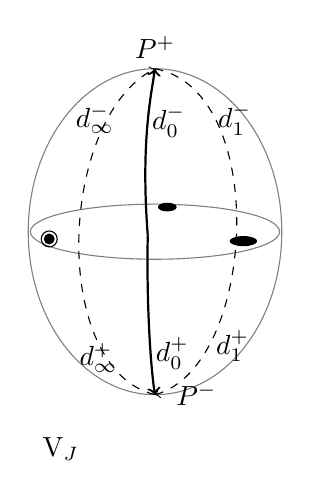
\begin{tikzpicture}[scale=.92]
\draw[gray] (0,0) ellipse (1.75 and 2.25);
\draw[gray] (0,0) ellipse (1.72 and .38);
\fill (-1.46,-.10) circle (.075);\draw (-1.46,-.10) circle (.11);
\fill (.17,.34) ellipse (.13 and .06);
\fill (1.22,-.13) ellipse (.19 and .07);
\draw[->,thick] (-.1,-.05).. controls (-.2,1.25) and (-.05,1.9)..(0,2.25);
\draw[->,thick] (-.1,-.05).. controls (-.12,-1.1) and (-.05,-1.95)..(0,-2.25);
\draw[dashed,->] (0,-2.25)..controls (-1.45,-1.9) and (-1.35,1.55)..(0,2.25);
\draw[dashed,->] (0,2.25)..controls (1.6,1.95) and (1.4,-1.85)..(0,-2.25);
\node[above] at (0,2.25) {$P^+$};\node[right] at (.16,-2.25) {$P^-$};
\node at (-.83,1.55) {$d_\infty^-$};\node at (.19,1.52) {$d_0^-$};\node at (1.1,1.55) {$d_1^-$};
\node at (-.78,-1.74) {$d_\infty^+$};\node at (.24,-1.68) {$d_0^+$};\node at (1.07,-1.58) {$d_1^+$};
\node at (-1.3,-3) {$\mathrm{V}_J$};
\end{tikzpicture}}
$\mathrm{IV}_J$, \deleted{formé des} \inserted{induit sur les} deux sommets $P^\omega$ \deleted{et $P^-$} $(\omega\in\uline{\omega})$, on peut le regarder comme le groupoïde libre engendré par le graphe de $=$ nom $\mathrm{V}_J$, ayant ces deux sommets, et trois arêtes --- donnant lieu aux six arcs $d_i^\omega$ avec $d_i^{\omega'}$ et $d_i^\omega$ opposés --- arcs permutés \deleted{\unsure{transitive}} \inserted{de façon} \deleted{\unsure{ment}} \inserted{simpl tr.} par \deleted{les} $G_J$. Un \deleted{autom.} \inserted{endom.} de ce groupoïde qui fixe les sommets est déterminé par les
\[
(46)\qquad u(\widetilde d_i^\omega)=\widetilde d_i^\omega\widetilde\psi_i^\omega(\widetilde\beta)
\qquad\text{avec }\widetilde\beta\in\widehat\Pi_{0,3}\quad\text{indépendant de }i,\omega
\]
La seule relation à satisfaire correspond aux équations $d_i^{\omega'}d_i^\omega=1$, qui donne
\[
(47)\qquad\widetilde\beta\sigma_\infty(\widetilde\beta)=1
\]
\figure{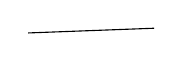
\begin{tikzpicture}\draw (0,0)--(1.6,.06);\end{tikzpicture}}

Considérons enfin le groupoïde induit sur les \deleted{pts} sommets $R_i^\omega,Q_i,P^\omega$ $(6+3+2=11\text{ sommets})$,
\margin{31}
